\documentclass[xetex,mathserif,serif]{beamer}
\usepackage{polyglossia}
\setdefaultlanguage[babelshorthands=true]{russian}
\usepackage{minted}
\usepackage{tabu}
\usepackage{graphicx}

\useoutertheme{infolines}

\usepackage{fontspec}
\setmainfont{FreeSans}
\newfontfamily{\russianfonttt}{FreeSans}

\definecolor{links}{HTML}{2A1B81}
\hypersetup{colorlinks,linkcolor=,urlcolor=links}

\setbeamertemplate{blocks}[rounded][shadow=false]
\setbeamercolor*{block title alerted}{fg=red!50!black,bg=red!20}
\setbeamercolor*{block body alerted}{fg=black,bg=red!10}

\tabulinesep=0.8mm

\title{Классификация текстового контента}
\author{Александр Смирнов и Федор Жилкин}
\date{24.05.2019г}

\begin{document}

	\frame{\titlepage}

	\begin{frame}
		\frametitle{Введение}
		\begin{figure}[h]
            \center{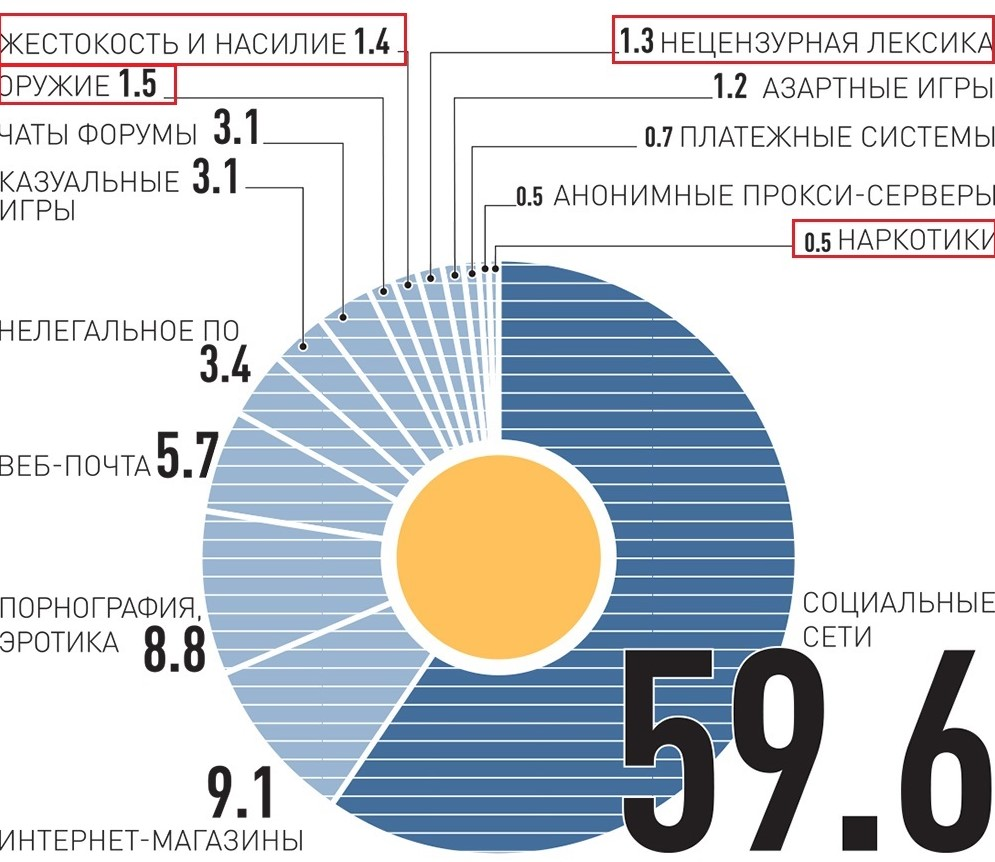
\includegraphics[scale=0.75]{images/children_statistics.jpg}}
        \end{figure}
	\end{frame}
	
	\begin{frame}
		\frametitle{Цели}
			\begin{itemize}
		 		\item Ограничить детей от взрослого текстового контента в интернете
				\item Получить опыт
    				\begin{itemize}
    			    	\item Бинарная классификация текста
    			    	\item Сбор данных для обучения
    			    	\item Написание Python-библиотеки
    			    	\item Написание расширения для Chrome
    			    	\item Написание Python-сервера для приёма запросов
    		    	\end{itemize}
			\end{itemize}
	\end{frame}
	
	\begin{frame}
		\frametitle{Сравнение с аналогами}
			\begin{itemize}
				\item Ограничения на поиск
					\begin{itemize}
				    	\item Семейный поиск Яндекс
				    	\item Безопасный поиск Google
			    	\end{itemize}
			    \item Контентная фильтрация
					\begin{itemize}
				    	\item Traffic Inspector
				    	\item Интернет Цензор
			    	\end{itemize}
			\end{itemize}
	\end{frame}
	
	\begin{frame}
		\frametitle{Сравнение с аналогами (2)}
		\begin{figure}[h]
            \center{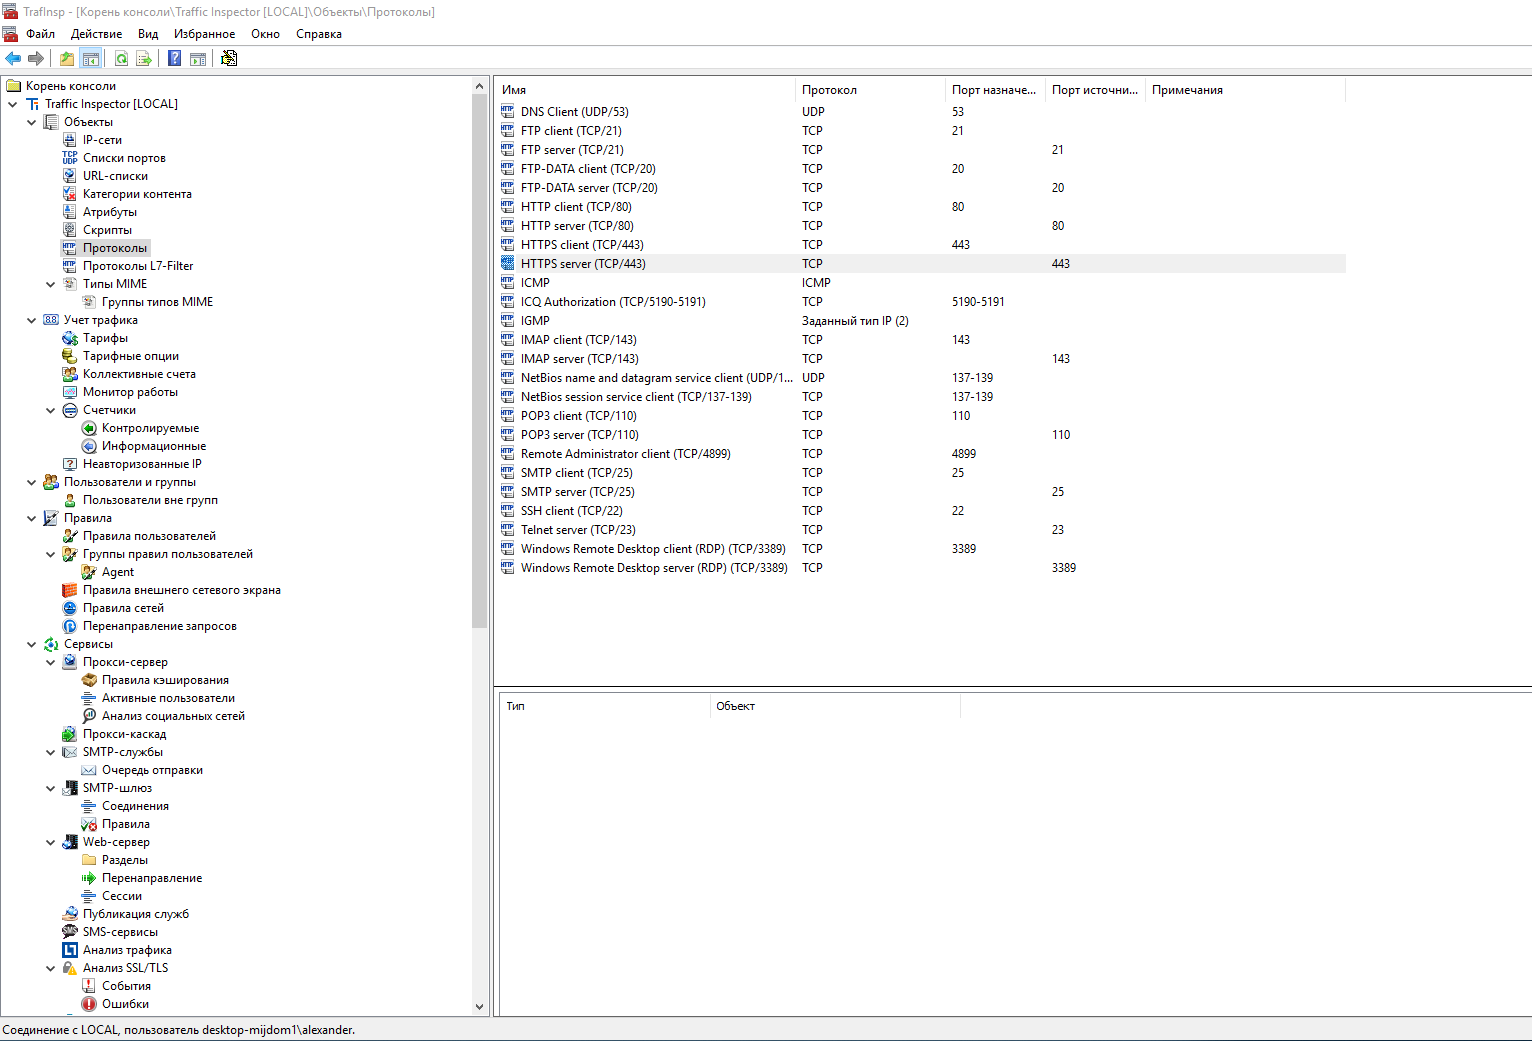
\includegraphics[scale=0.22]{images/bad_interface.png}}
            \caption{Пример интерфейса схожей программы}
            \label{fig:image}
        \end{figure}
	\end{frame}	
	
	\begin{frame}
		\frametitle{Задачи}
			\begin{itemize}
		 		\item Провести анализ возможных решений для классификации текста
		 		\item Собрать рассказы для взрослых и обычные рассказы
		 		\item Написать Python-сервер, использующий обученную модель для ответа на запросы от расширения
		 		\item Сделать расширение для Chrome, обращающееся к серверу
			\end{itemize}
	\end{frame}	
	
	\begin{frame}
		\frametitle{Сбор данных}
		\begin{itemize}
			\item Рассказы для взрослых берём с сайта ideer.ru
			\item Рассказы для широкого круга читалей берём с множества сайтов по разным тематикам
		\end{itemize}
	\end{frame}		
	
	\begin{frame}
		\frametitle{Анализ подходов к классификации текста}
		\begin{itemize}
			\item Rule-based
			\item Machine Learning based
			\item Hybrid systems
		\end{itemize}
	\end{frame}	
	
	\begin{frame}
		\frametitle{Характеристики сравнения эффективности}
		\begin{itemize}
			\item Accuracy – общая точность классификатора
			\item Recall – отношение заблокированных взрослых сайтов к общему количеству взрослых сайтов (\% классифицированных взрослых сайтов)
			\item Precision – отношение заблокированных взрослых сайтов к числу всех заблокиронных сайтов (точность блокировки)
			\item F1 Score – среднее гармоническое между Precision и Recall, для учёта и того, и другого в одной величине
		\end{itemize}
	\end{frame}
	
	\begin{frame}
		\frametitle{Сравнение}
    		\begin{itemize}
    			\item Random model – случайный выбор блокировать/не блокировать
    			\item Rule-based model – блокировка по списку непотребных слов
    			\item Classifier – 3-х слойная обычная сеть
    			\item Upgraded Classifier – Classifier, из словаря которой были исключены самые частые слова и добавлена ненормативная лексика
    		\end{itemize}
            \begin{table}[]
            \begin{tabular}{|l|l|c|c|c|}
            \hline
                                         & F1 Score      & Accuracy & Recall & Precision \\ \hline
            Random model                 & 0.58          & 0.51     & 0.58   & 0.58      \\ \hline
            Rule-based model             & 0.06          & 0.41     & 0.03   & 1.0       \\ \hline
            Classifier                   & 0.90          & 0.88     & 0.93   & 0.87      \\ \hline
            \textbf{Upgraded Classifier} & \textbf{0.91} & 0.90     & 0.92   & 0.91      \\ \hline
            \end{tabular}
            \end{table}

	\end{frame}		
	
	\begin{frame}
		\frametitle{Результаты обучения}
	    	\begin{columns}[t]
                \column{.3\textwidth}
                    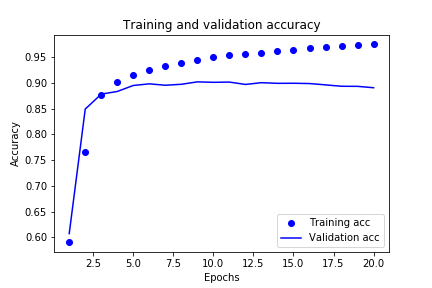
\includegraphics[scale=0.37]{images/acc.png}
                \column{.3\textwidth}
                    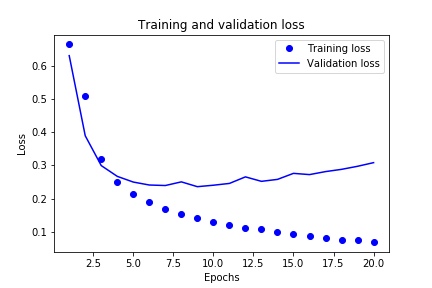
\includegraphics[scale=0.37]{images/loss.png}
                \column{.05\textwidth}
            \end{columns}
	\end{frame}		
	
	\begin{frame}
		\frametitle{Взаимодействие расширения и сервера}
	    	\begin{figure}[h]
            \center{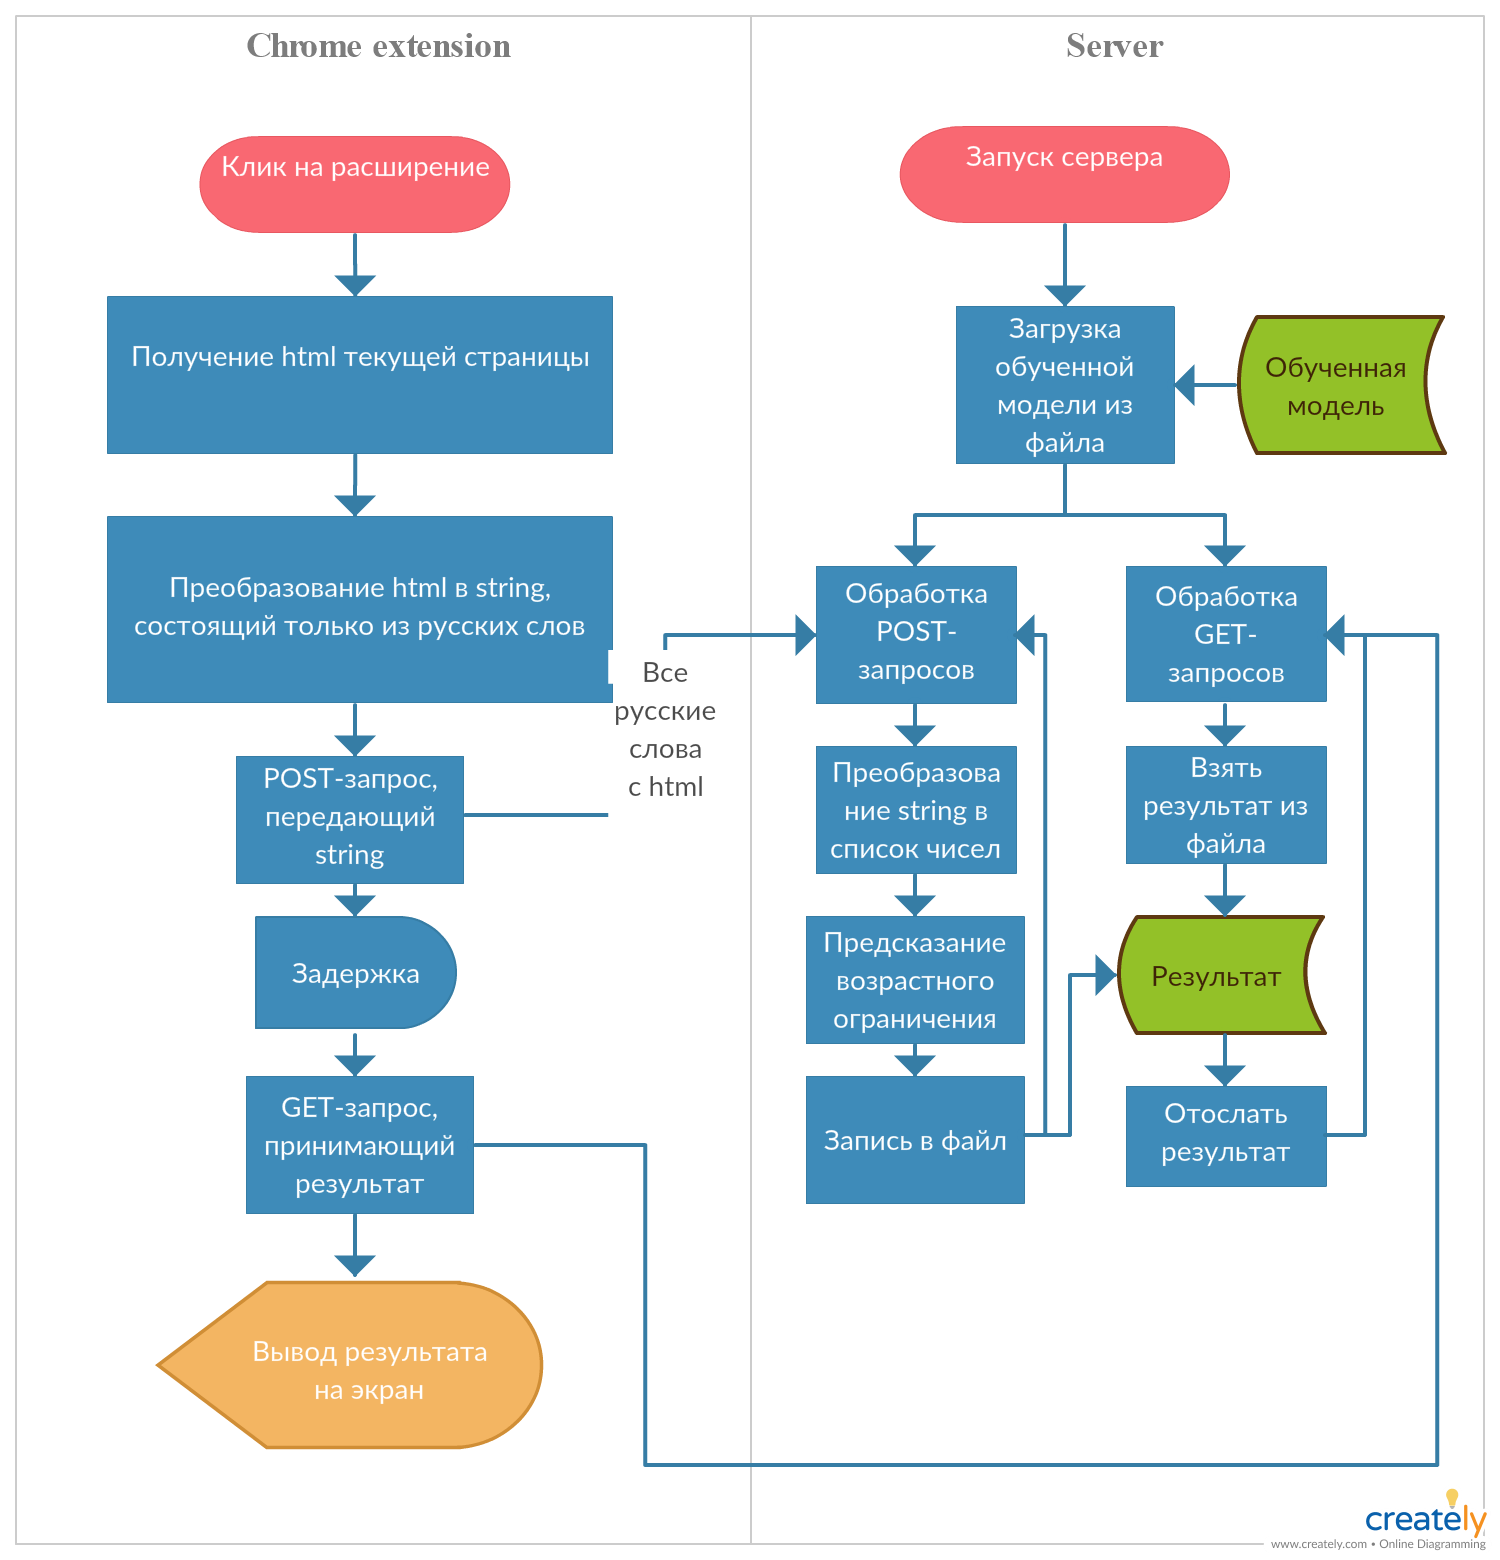
\includegraphics[scale=0.13]{images/uml.png}}
        \end{figure}
	\end{frame}		
	
	\begin{frame}
		\frametitle{Итоги}
		\begin{itemize}
			\item Федор
			    \begin{itemize}
			    	\item Сбор данных
			    	\item Библиотека
		        \end{itemize}
			\item Александр
			    \begin{itemize}
			    	\item Классификация текста
			    	\item Сервер
			    	\item Расширение
		        \end{itemize}
		\end{itemize}
	\end{frame}
	
	\begin{frame}
		\frametitle{Результаты}
		\begin{itemize}
			\item Сделано расширение для Chrome – \url{https://github.com/SmirnovAlexander/PoemClassifier}
			\item Сделана библиотека на pypi – \url{https://pypi.org/project/TalesParse/}
			\item Собраны рассказы на kaggle – \url{https://www.kaggle.com/idoldev/adult-and-child-russian-tales-dataset-with-label}
			\item Написан сборщик рассказов – \url{https://github.com/Feodoros/Scraping_Tales}
		\end{itemize}
	\end{frame}

\end{document}